\documentclass[11pt,twocolumn,notitlepage,openany,twoside]{book}
\usepackage[paperheight=11.25in,paperwidth=8.75in, margin=0.625in]{geometry}
\usepackage{titlesec}
\usepackage{verbatim}
\pagestyle{headings}

% Figure setup
\usepackage[]{graphicx}
\graphicspath{ {figures/} }
\usepackage{float}
\setlength{\floatsep}{0pt plus 2.0pt minus 2.0pt}
\setlength{\dbltextfloatsep}{5pt plus 2.0pt minus 2.0pt}
\usepackage{caption}

% % Table setup
% \usepackage[table]{xcolor}
% \usepackage{array}
% \newcolumntype{L}[1]{>{\raggedright\let\newline\\\arraybackslash\hspace{0pt}}m{#1}}
% \usepackage{multirow}
%
% \newcommand*{\tabbox}[2][t]{%
%     \vspace{0pt}\parbox[#1][1.7\baselineskip]{8pt}{\strut#2\strut}}
%
% \newcommand*{\tabboxb}[2][t]{%
%     \vspace{0pt}\parbox[#1][2.2\baselineskip]{8pt}{\strut#2\strut}}

% Remove the giant space at the beginning of a chapter
\titleformat{\chapter}[display]
    {\normalfont\huge\bfseries}{\chaptertitlename\ \thechapter}{20pt}{\Huge}
\titlespacing*{\chapter}{0pt}{0pt}{20pt}

\title{Metabolic interactions and capabilities within microbial communities}
\author{Gregory Leonard Medlock}


% % Optimization problem formatting
% \usepackage{amsmath}
%
% % Bibliography setup
% \usepackage[backend=biber, style=numeric-comp,sorting=none,terseinits=true, giveninits=true,maxbibnames=4]{biblatex}
% \addbibresource{rf_references.bib}
% \DeclareNameAlias{default}{last-first}
% \renewcommand*{\revsdnamepunct}{}
% \renewcommand*{\bibfont}{\small}

\begin{document}
\frontmatter

\begingroup
\let\clearpage

\tableofcontents
\hspace{1.5cm}
\listoffigures
\hspace{1.5cm}
\listoftables

\endgroup

\clearpage
\addcontentsline{toc}{chapter}{Acknowledgments}
\section*{Acknowledgments}

Acknowledgements will be here

\mainmatter


%------------------------------------------------------------------------------------
% Chapter 1 Introduction
%------------------------------------------------------------------------------------
\chapter{Introduction}
%\begin{refsection}

\section{Specific Aims}

These the aims:

\begin{enumerate}
  \item \textbf{Aim 1: Identify \textit{in vitro} metabolic interactions between members of a defined mouse microbiota}. Aim 1
  \item \textbf{Aim 2: Develop an ensemble-driven framework for the refinement and application of genome-scale metabolic network reconstructions of gut microbes}. Aim 2
\end{enumerate}



\section{A Preview of this Dissertation}

Preview text

%\end{refsection}

%------------------------------------------------------------------------------------
% Chapter 2
%------------------------------------------------------------------------------------
\chapter{Inferring Metabolic Mechanisms of Interactions within a Defined Gut Microbiota}
\chaptermark{Metabolic interactions}

%\begin{refsection}

The contents of this chapter are published as a research article here:

\medskip\noindent
Medlock GL, MA Carey, DG McDuffie, MB Mundy, N Giallourou, JR Swann, GL Kolling, JA Papin. (2018). Inferring Metabolic Mechanisms of Interactions within a Defined Gut Microbiota. \textit{Cell Systems}, 7(3):p245-357.e7.

\section{Context}

\section{Synopsis}

\section{Introduction}

Text from paper

\section{Methods}
\subsubsection{A methods subsection}
This is in the subsection

\section{Results}
\subsubsection{A results subsection}
This is in the subsection

\begin{figure*}
\centering
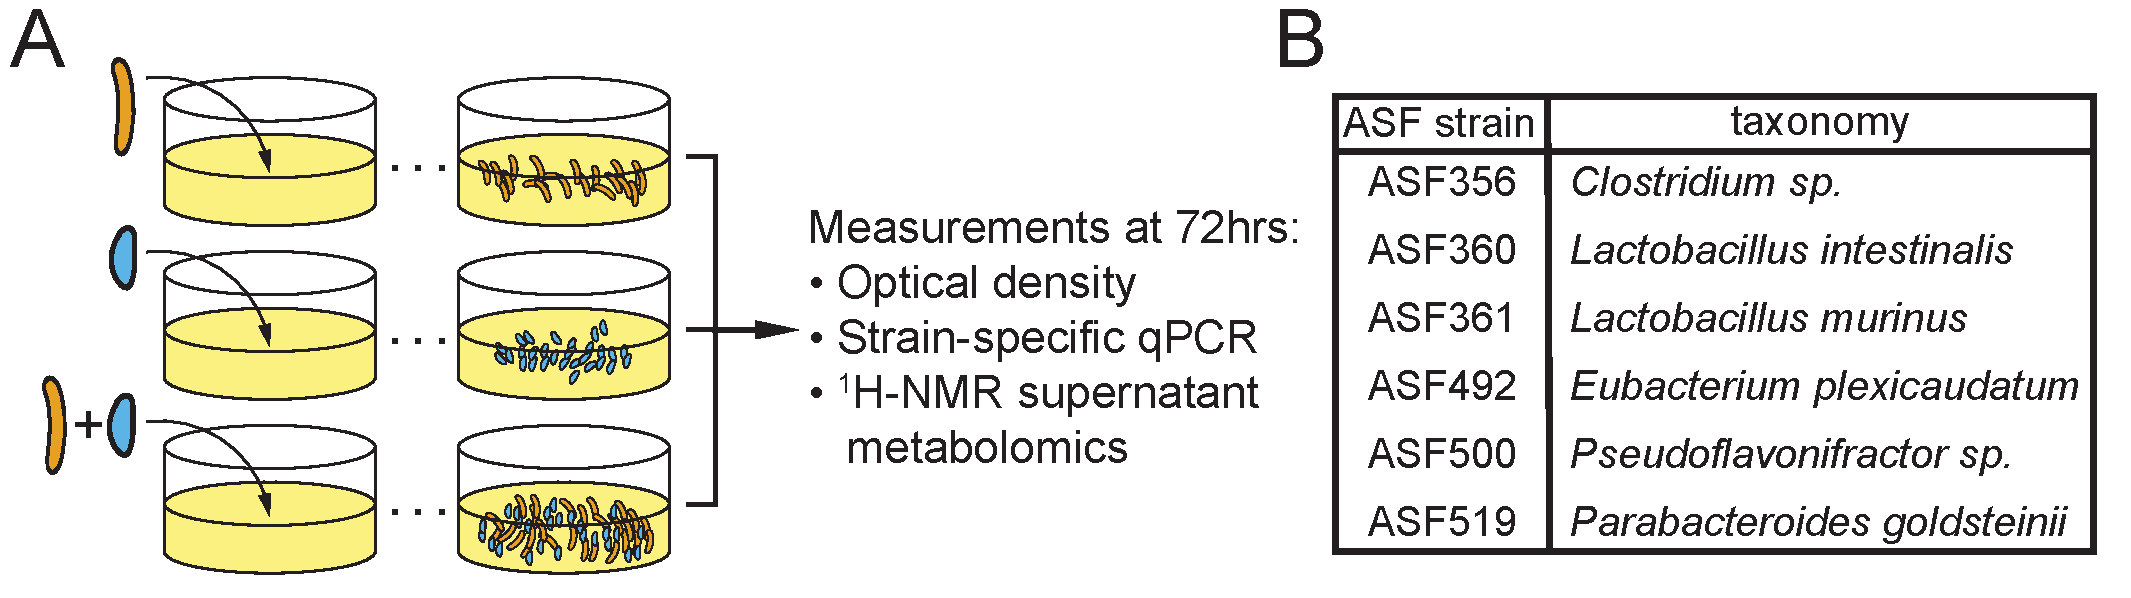
\includegraphics[width=0.8\textwidth]{ch2_fig1}
\caption[Summary of co-culture experiment design, measurements, and total growth outcomes in monocultures and co-cultures.]{\textbf{Summary of co-culture experiment design, measurements, and total growth outcomes in monocultures and co-cultures.} \textbf{A)} Experimental procedure for each pair of strains and measurements taken. \textbf{B)} Taxonomic assignment for strains included in this study.}
\end{figure*}


\begin{figure*}
\centering
\includegraphics[width=0.8\textwidth]{ch2_fig2}
\caption[The effects of pairwise co-culture on the abundance of each strain.]{\textbf{The effects of pairwise co-culture on the abundance of each strain.} \textbf{A)} Relative abundance of each strain in monoculture and co-culture determined via qPCR. Abundance is plotted on linear scale, not log-transformed. x-axis describes abundance of strain at the bottom of the column; y-axis describes abundance of strain left of each row. Diamonds indicate abundance of each strain in monoculture, with mean shown by a dashed line. Abundance of each strain in co-culture as indicated by the row and column labels is shown by a black circle, with mean abundances indicated by grey dashed lines. Abundance for each strain is z-score normalized using mean and standard deviation of monoculture abundance to center and scale the data, respectively. N=9 for all samples except for those with Pseudoflavonifractor ASF500 or Eubacterium ASF492, for which N=6. \textbf{B)} Heatmap of mean abundance of each strain in co-culture relative to monoculture. Blue indicates less abundant, while red indicates more abundant, than monoculture. The upper left and lower right triangles in each square describes abundance of the strain labelled on the left of row and bottom of column, respectively. White circles indicate differential abundance between monoculture and co-culture (\textit{p} < 0.10, Mann-Whitney U test with false discovery rate correction using Benjamini-Hochberg procedure). \textbf{C)} Summary of interspecies interactions. Non-zero interactions in the triangular matrix indicate significant differential abundance as shown in Figure 2B.}
\end{figure*}


\begin{figure*}
\centering
\includegraphics[width=0.8\textwidth]{ch2_fig3}
\caption[Metabolic behavior of each strain in monoculture and emergent behavior in co-cultures.]{\textbf{Metabolic behavior of each strain in monoculture and emergent behavior in co-cultures.} \textbf{A)} Heatmap describing supernatant metabolomes for each monoculture. Red/blue indicate higher/lower concentrations than fresh medium, respectively. Values are centered at 0 using the mean in fresh media, then scaled between -1 and +1 by dividing by the maximum change in concentration for each metabolite in any sample in the study. Unnamed metabolites not shown. Hierarchical clustering was performed using Euclidean distances and complete linkage. \textbf{B-E)} Principal component analysis (PCA) of monocultures and co-culture, performed independently for each subplot. Sky blue/orange circles correspond to monoculture supernatant metabolomes from strain labelled with same color. Co-culture samples for the two strains in each subplot title are indicated by grey circles. Percent variance captured by each principal component is labelled on each axis.}
\end{figure*}


\begin{figure*}
\centering
\includegraphics[width=0.8\textwidth]{ch2_fig4}
\caption[Accounting for co-culture growth outcomes with ConYE to identify emergent metabolism.]{\textbf{Accounting for co-culture growth outcomes with ConYE to identify emergent metabolism.} \textbf{A)} Procedure for the constant yield expectation (ConYE) model. \textbf{B)} Examples of ConYE results for Lactose, Lactate, Valine, and Proline. Diagonal shows monoculture behavior for each strain. Every pair of triangles indicates the observed metabolite abundance in co-culture (lower left), the expected metabolite abundance (upper right), and whether there was a significant difference between observed and expected values. Centering and scaling performed as in Figure 3, except expected values were included while selecting a max value. Mann-Whitney U-Test with false discovery rate (FDR) control using the Benjamini-Hochberg procedure was performed for all 1290 comparisons (15 co-cultures, 86 metabolites each). Asterisk indicates p < 0.05 for the metabolite in the co-culture containing the indicated strains. \textbf{C)} ConYE results for all strain pairings for metabolites that were consumed by one or both strains in monoculture (left, blue), produced by one or both strains in monoculture (middle, red), or produced by one strain in monoculture and consumed by the other strain in monoculture (right, green). Each point represents a metabolite in a co-culture pair. x axis show the difference between observed and expected metabolite abundance in co-culture (scaled as in panel B), and y axis shows the p-value from ConYE. Points above grey line have p < 0.05. Percentage of points in the labelled quadrant relative to the rest of the points in the subplot is shown.}
\end{figure*}


\begin{figure}[tb]
\centering
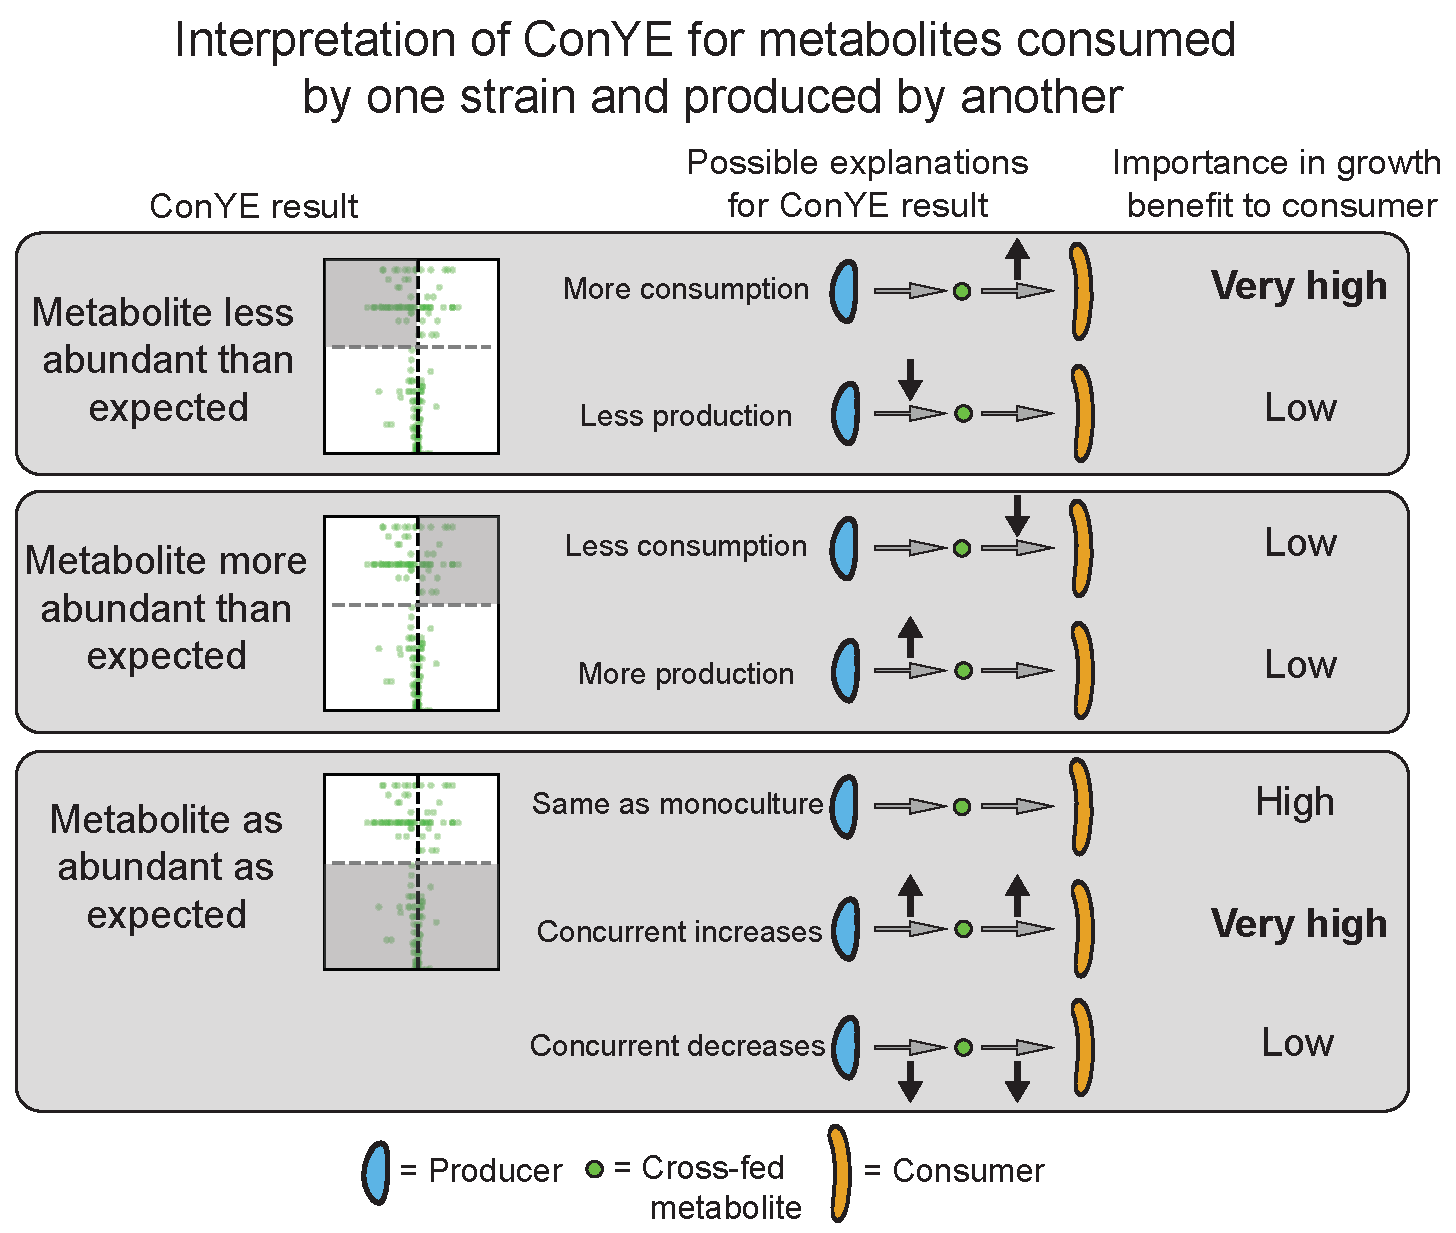
\includegraphics[width=\linewidth]{ch2_fig5}
\caption[Interpretations of ConYE results for metabolites consumed by one strain in monoculture and produced by another strain in monoculture.]{\textbf{Interpretations of ConYE results for metabolites consumed by one strain in monoculture and produced by another strain in monoculture.} In this example, the consumer experienced a growth benefit. The shaded region of each volcano plot describes the points that fall into the category described on left. In “Importance in growth benefit to consumer” column, the entry for each scenario assumes that consumption of the metabolite is coupled with biomass production. The importance assignments are qualitative, and reflect whether the consumer experienced an increase in metabolite flux in the explanatory scenario (high for increased flux, low for decreased flux).}
\end{figure}


\begin{figure*}
\centering
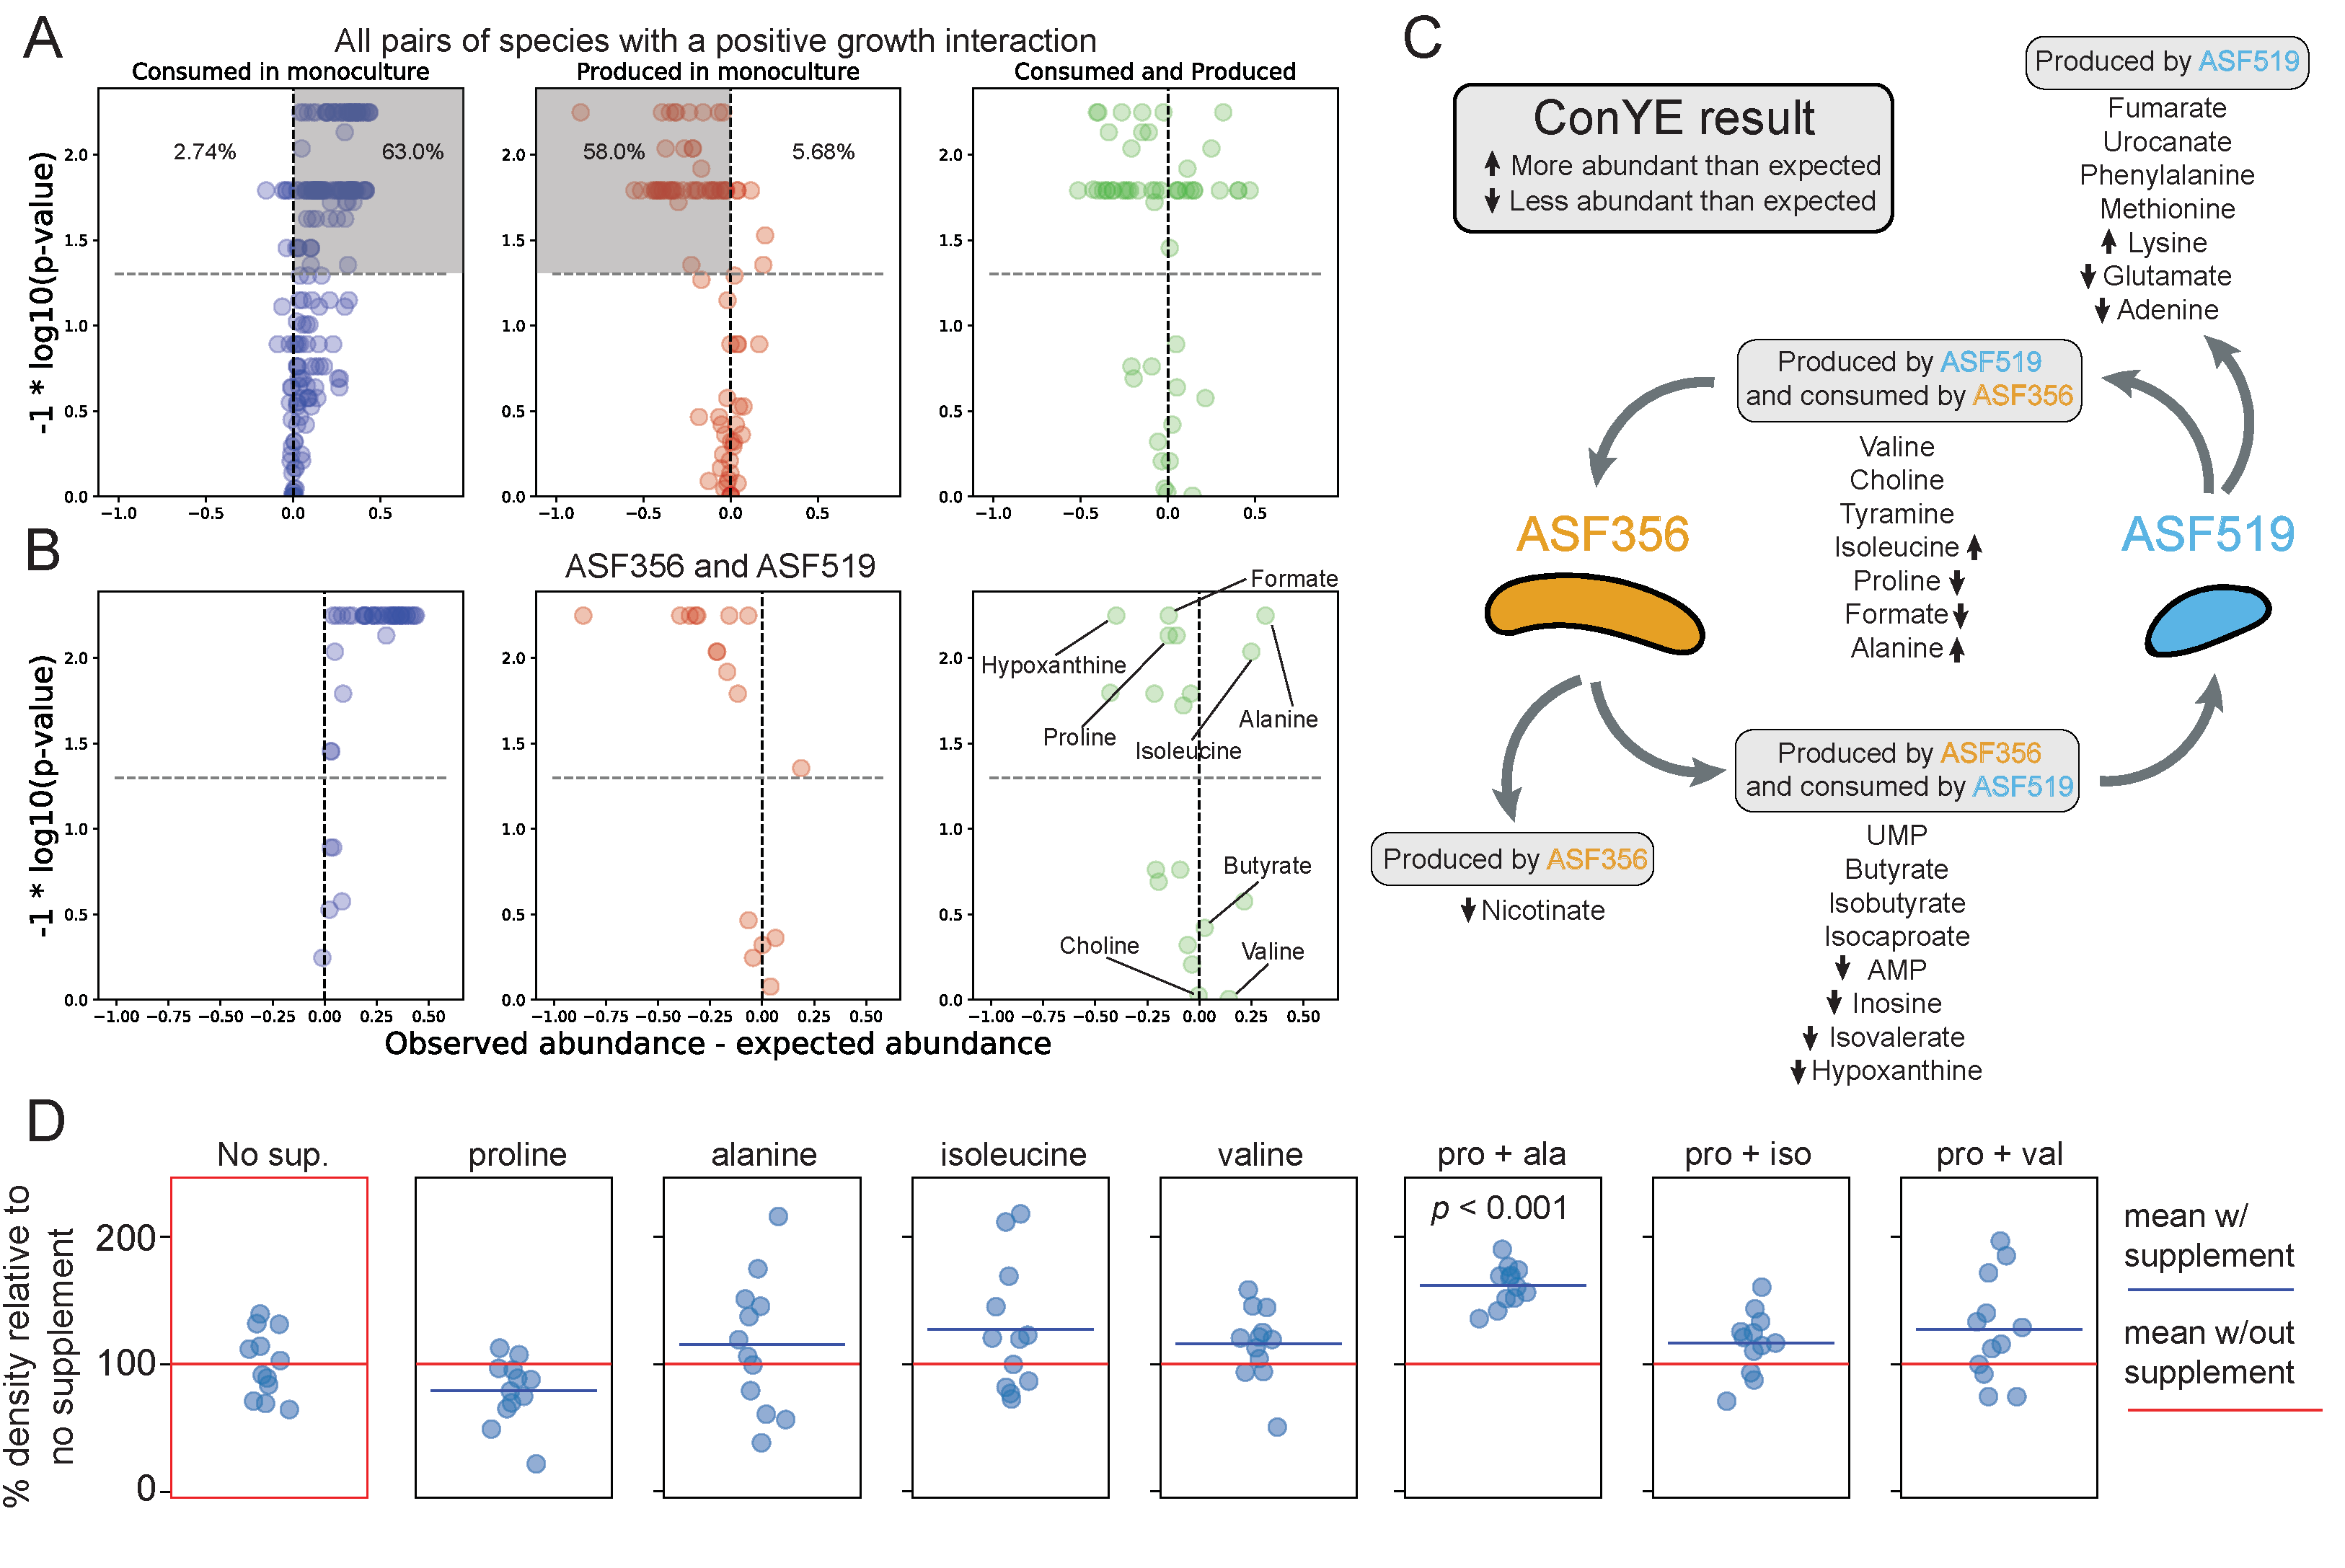
\includegraphics[width=0.9\textwidth]{ch2_fig6}
\caption[Emergent metabolism in co-culture pairings with a growth benefit and in vitro testing.]{\textbf{Emergent metabolism in co-culture pairings with a growth benefit and in vitro testing.} \textbf{A)} ConYE results for all metabolites from co-cultures with a positive growth interaction. Shaded quadrants represent consumed metabolites that were more abundant than expected (left) or less abundant than expected (middle). Percentages shown represent the number of metabolites within the plot that fall in the quadrant. \textbf{B)} ConYE results for co-culture of Clostridium ASF356 and Parabacteroides ASF519. Metabolites on right for which p > 0.05 are labeled unless they could not be assigned an identity. Metabolites for which p < 0.05 are labeled if assigned an identity and abs(x) > 0.10 for that metabolite. x and y axes are scaled as in Figure 4. \textbf{C)} Metabolic interaction topology for Clostridium ASF356 and Parabacteroides ASF519. ConYE results are indicated with arrows pointing up or down for metabolites for which the null hypothesis was rejected. Metabolite classifications are based on monoculture behavior. \textbf{D)} OD600 of Clostridium ASF356 monocultures after 72 hours of growth in supplemented media conditions. ”No sup.” had no supplement added, while conditions with a single amino acid were supplemented at 1.25g/L. In conditions with two supplements, each metabolite is supplemented at 1.25g/L. “pro + ala”, “pro + iso”, and “pro + val” conditions include L-proline with L-alanine, L-isoleucine, or L-valine, respectively.}
\end{figure*}

\section{Discussion}

Text from paper

\section{Conclusion}

new conclusion section

\section{Acknowledgments}

Acknowledgements

\section{References}

%\end{refsection}



\end{document}
